\chapter{Derivative of the Contrast Metric}\label{sec:jacobian}
Since we use bilinear voting to evaluate the \textit{dirac delta}, the
derivatives of the cost function \cref{eq:variance} can be
analytically computed as
\begin{align}
  \intertext{Let}
  \rho\left(\vec{x};\bm{\theta}\right)&=\mathcal{I}\left(\vec{x};\bm{\theta}\right)-\mu\left(\mathcal{I}\left(\vec{x};\bm{\theta}\right)\right)\\
  \intertext{Then}
  \frac{\partial}{\partial\bm{\theta}}\mathrm{Var}\left(\mathcal{I}\left(\vec{x};\bm{\theta}\right)\right)&=\frac{2}{\mid\Omega\mid}\int_{\Omega}\rho\left(\vec{x};\bm{\theta}\right)\frac{\partial\rho\left(\vec{x};\bm{\theta}\right)}{\partial{\bm{\theta}}}d\vec{x}    \label{eq:dVdw}
\end{align}
The derivatives of the warped image are
\begin{equation}
  \label{eq:dIdw}
  \frac{\partial\mathcal{I}\left(\vec{x};\bm{\theta}\right)}{\partial{\bm{\theta}}}=-\sum_{k=1}^N\pm_k\nabla\delta\left(\vec{x}-\vec{x}'_k\left(\bm{\theta}\right)\right)\frac{\partial\vec{x}'_k\left(\bm{\theta}\right)}{\partial\bm{\theta}},
\end{equation}
In the case of planar homography the events warping is computed as
\begin{align}
  \bm{\theta}&=\left(\bm{\omega}^\top,\vec{v}^\top,\varphi,\psi\right)^\top\in\mathbb{R}^8\\
  \vec{x}'_k\left(\bm{\theta}\right)&=
                                      \begin{bmatrix}
                                        x'_{im}&y'_{im}&1
                                      \end{bmatrix}^\top=
                                                         \begin{bmatrix}
                                                           x'/z'&y'/z'&1
                                                         \end{bmatrix}^\top\\
  \bar{\vec{x}}'_k\left(\bm{\theta}\right)&=
                                            \begin{bmatrix}
                                              x'&y'&z'
                                            \end{bmatrix}^\top\nonumber\\&=
  \mat{P}\left(\mat{R}(t)^\top\left(\mat{I}+\vec{T}(t)\vec{n}^\top/d\right)\right)^{-1}\vec{x}_k\nonumber\\
             &=
               \mat{P}\left(\mat{I}+\vec{v}t\vec{n}^\top\right)^{-1}\mat{R}(t)\vec{x}_k, \label{eq:x_x}
               % &=
               % \mat{P}\left(\mat{I}-\frac{\vec{v}t\vec{n}^\top}{\vec{n}^\top\vec{v}t+1}\right)\mathrm{exp}(\bm{\omega}^\wedge
               % t)\vec{x}_k,
\end{align}
where $\mat{P}$ is the projection matrix from the camera frame to the
world frame or the map. Also, for simplicity of notation we assume
$d = 1$, and denote
$\mat{P}\left(\mat{I}+\vec{v}t\vec{n}^\top\right)^{-1}$ as
$\mat{P_v}$. Since $t$ usually spans a small temporal window, we can
simplify the derivative with respect to angular velocity as
\begin{align}
  \mat{R}(t)& =\mathrm{exp}(\bm{\omega}^\wedge t)\approx\mat{I}+\bm{\omega}^\wedge t\\
  \frac{\partial\bar{\vec{x}}'_k}{\partial\bm{\omega}}&=-\mat{P_v}t\vec{x}_k^\wedge.  \label{eq:dxdo}
\end{align}
The above equation makes use of the equivalence
$\bm{\omega}\times\vec{x}_k=-\vec{x}_k\times\bm{\omega}$.

The derivative with respect to the linear velocity is
\begin{align}
  \frac{\partial\bar{\vec{x}}'_k}{\partial\vec{v}}&=-\frac{t\vec{n}^\top\mat{R}(t)\vec{x}_k}{\vec{n}^\top\vec{v}t+1}\mat{P_v} \label{eq:dxdv}\\
  eu
\end{align}
Similarly we have
\begin{align}
  \frac{\partial\bar{\vec{x}}'_k}{\partial\vec{n}}&=-\frac{t\vec{v}^\top\mat{R}(t)\vec{x}_k}{\vec{n}^\top\vec{v}t+1}\mat{P_v} \\
  \intertext{and}
  \frac{\partial\bar{\vec{x}}'_k}{\partial(\varphi;\psi)}&= \frac{\partial\bar{\vec{x}}'_k}{\partial\vec{n}}\frac{\partial\vec{n}}{\partial(\varphi;\psi)},\\
  \intertext{with}
  \frac{\partial\vec{n}}{\partial(\varphi;\psi)}&=
                                                  \begin{bmatrix}
                                                    -\sin\varphi\sin\psi&\cos\varphi\cos\psi\\
                                                    \cos\varphi\sin\psi&\sin\varphi\cos\psi\\
                                                    0&-\sin\psi
                                                  \end{bmatrix}
                                                       \label{eq:dvdn}
\end{align}
With the above quantities
\begin{equation*}
  \label{eq:dx_dtheta}
  \frac{\partial\bar{\vec{x}}'_k}{\partial\bm{\theta}}=
  \begin{bmatrix}
    \frac{\partial\bar{\vec{x}}'_k}{\partial\bm{\omega}}&
    \frac{\partial\bar{\vec{x}}'_k}{\partial\vec{v}}&
    \frac{\partial\bar{\vec{x}}'_k}{\partial\varphi}&\frac{\partial\bar{\vec{x}}'_k}{\partial\psi}
  \end{bmatrix}\in\mathbb{R}^{3\times8}
\end{equation*}
we can compute the gradient
$\frac{\partial\vec{x}'_k}{\partial\bm{\theta}}$ as
\begin{equation}
  \label{eq:dxdtheta}
  \frac{\partial\vec{x}'_k}{\partial\bm{\theta}}=\frac{\partial\bar{\vec{x}}'_k}{\partial\bm{\theta}}\frac{1}{z'}-\bar{\vec{x}}'_k\frac{\partial z'}{\partial\bm{\theta}}\frac{1}{z'^2}
\end{equation}
Theoretically, the derivative of the Dirac delta
$\nabla\delta(\vec{x})$ should be evaluated at each pixel location
($240\times180$ for DAVIS) for each event. However, since we are using
bilinear voting, a infinitesimal change $d\vec{x}$ at an event
location $\vec{x}$ will only affect the derivative evaluated at the
four neighboring pixels of $\vec{x}$. An illustration is shown in
\cref{fig:bi_voting}

\begin{figure}
  \begin{minipage}[t]{0.48\textwidth}
    \centering 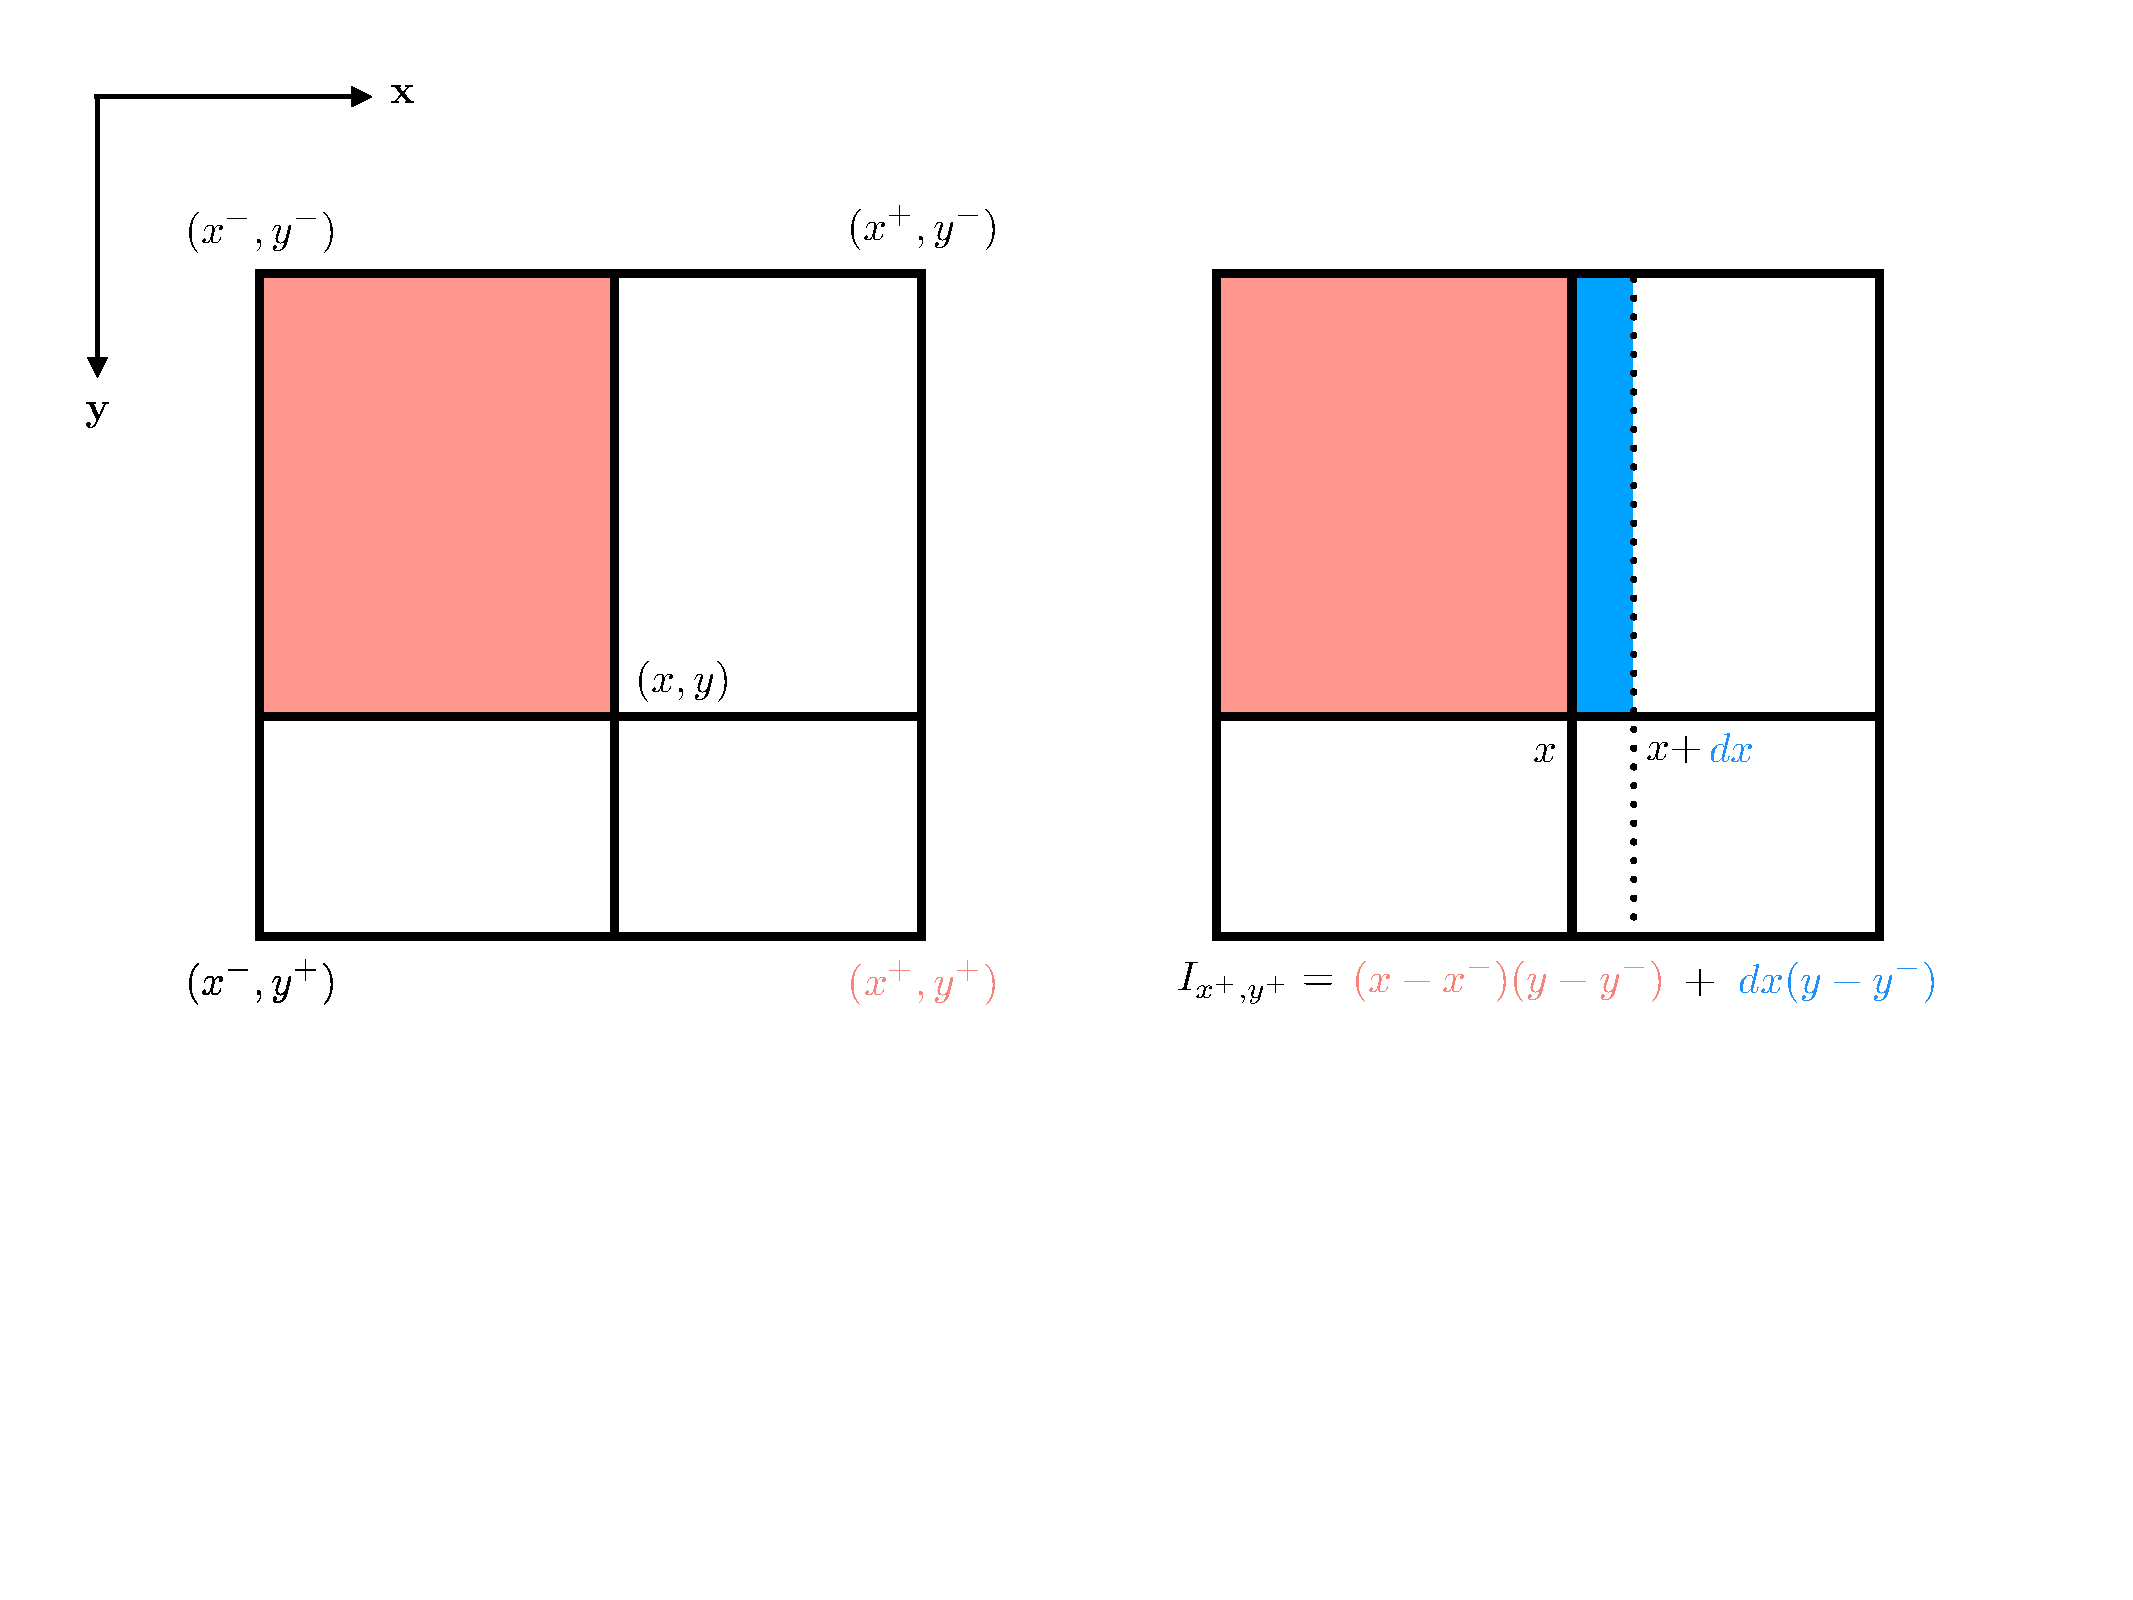
\includegraphics[width =
    \textwidth]{images/bi_voting.pdf} (a) The intensity at a pixel
    location is the area of the rectangle spanned by the opposite
    pixel and the event location
  \end{minipage}
  \hfill
  \begin{minipage}[t]{0.48\textwidth}
    \centering 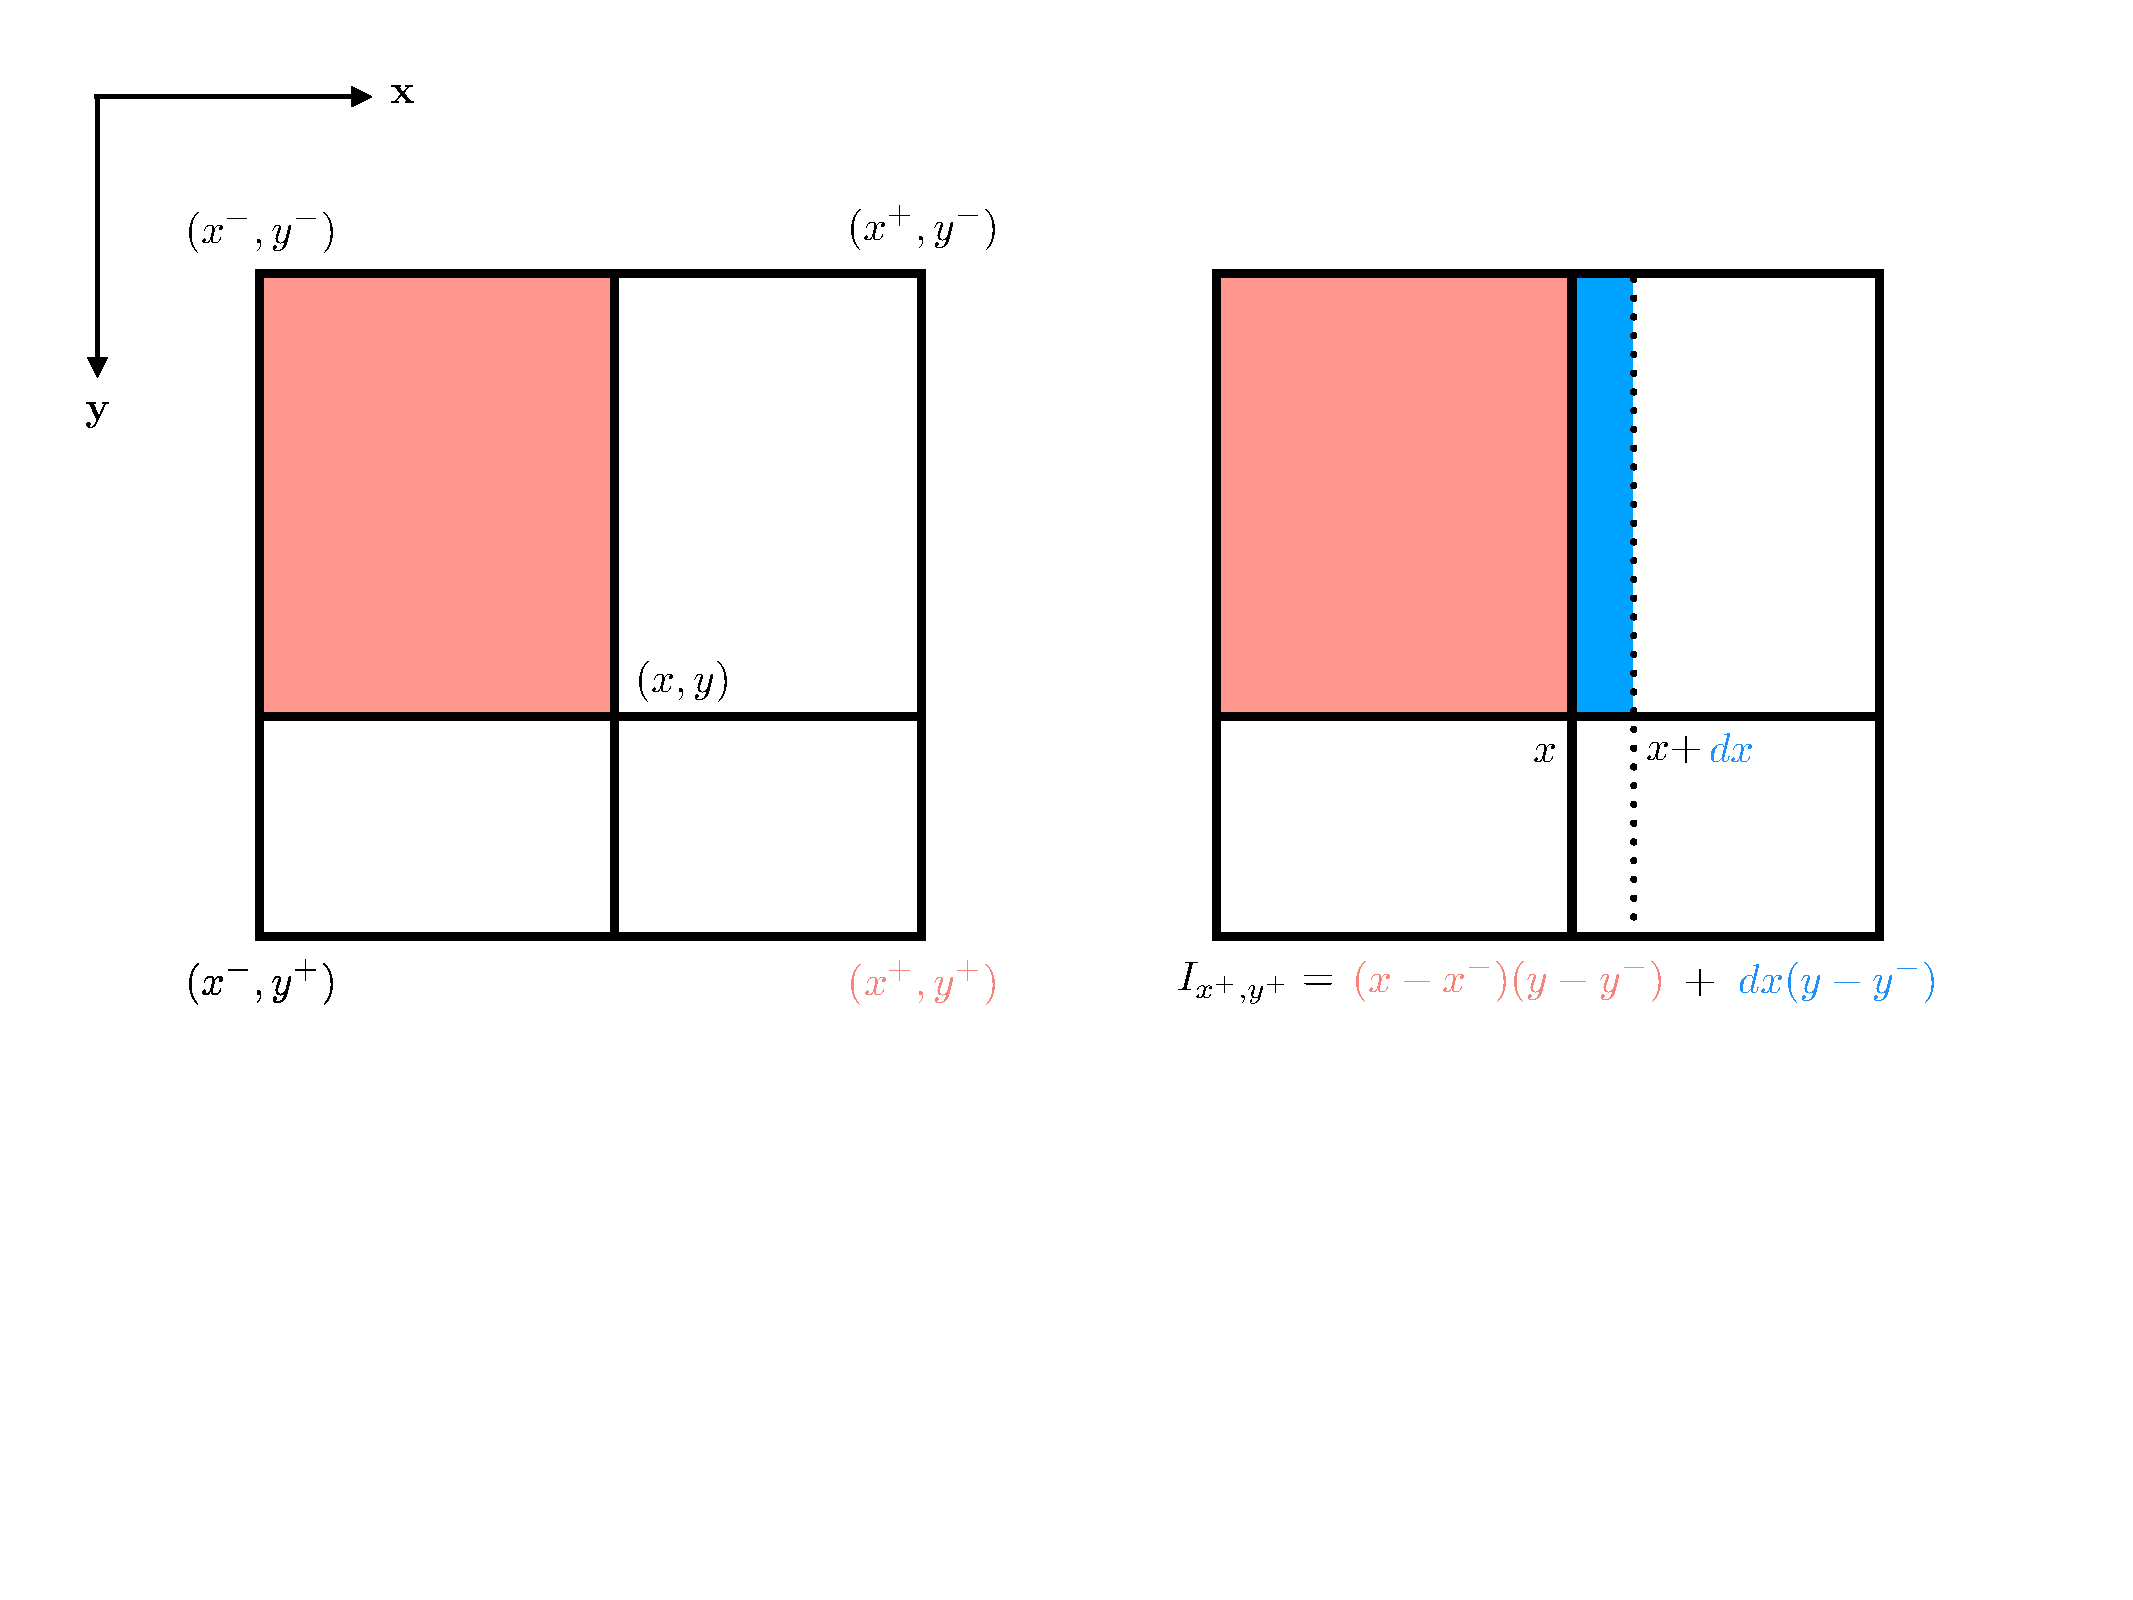
\includegraphics[width =
    \textwidth]{images/bi_voting.pdf} (b) Intensity change after an
    infinitesimal movement of the event
  \end{minipage}
  \caption{Bilear voting.}
  \label{fig:bi_voting}
\end{figure}
The detailed algorithms for the evaluation of the Dirac delta as well
as its derivative is shown below
\Input{A set of warped events $\mathscr{E}*\{e'_k\}_1^N$}
\Output{The intensity at each pixel &\mathcal{I}(\vec{x})& as well as the derivative $\frac{\partial\mathcal{I}(\vec{x})}{\partial\vec{x}}$}
Remap $L_{k-1}(\vec{u})$ to current pose and update $R_{k-1}(\vec{u})$  to get $L_k(\vec{u}),R_k(\vec{u})$ \;
\ForEach{voxel block VB requested during swap-in}{
	\ForEach{voxel in VB}{
		get voxel global location $\vec{x}_{v,g}=h.\vec{pos}+\vec{x}_{v,VB}$\;
		forward project $v$ to image plane with $\vec{u}=\pi\left(KT_{d,g}^{-1}\tilde{\vec{x}}_{v,g}\right)$\;
		\If{$\vec{u}$ in current image}{
			\uIf{$L_k(\vec{u})$ empty}{
				$L_k(\vec{u})=\vec{x}_{v,g}+\mu.sdf.\vec{r}$\;
				$R_k(\vec{u})=v.reliability$\;
				}
				\ElseIf{$v.reliability>R_k(\vec{u})$}{
				$v.reliability=L_k(\vec{u})$\;
				}
		}
	}
}
\caption{sIncremental Raycasting}
\end{algorithm}
\BlankLine

However, a general nonlinear optimization is usually very hard,
especially at bundle adjustment stage he jacobian matrix only measures
the local grad
